\documentclass[portrait,a0,final]{a0poster}
\usepackage{booktabs, tikz, multicol, float, subcaption}
\usetikzlibrary{arrows}
\usepackage[english]{babel}
\floatplacement{figure}{H}
\floatplacement{table}{H}
\usepackage[margin={6cm,6cm}]{geometry}
\usepackage[parfill]{parskip}  %avoid indenting first line of paragraph
\usepackage{enumitem} 
\setlist[enumerate]{itemsep=0mm}
 
\begin{document}
\bibliographystyle{CIM14}
\normalsize \color{black}\sffamily %default font size

% TITLE
%%%%%%%%%%%%%%%%%%%%%%%%%%%%%%%%%%%%%%%
\begin{center}                
\veryHuge \color{red}
%%%%%%%%%%%%%%%%%%%%%%%%%%%%%%%%%%%%%%%
\textbf{Haptic pattern representation using music technologies}\\
\end{center}
\vspace{2cm}

%\begin{multicols}{2}
%%%%%%%%%%%%%%%%%%%%%%%%%%%%%%%%%%%%%%%
% AUTHORS
\begin{figure}[H]
    %\begin{center}
        
\includegraphics[width=0.15\textwidth]{graphics/OCAD_Logo.png}
    %\end{center}
    %\caption{\label{fig:arrowsMoving00}}
\end{figure}

\normalsize \color{black}
%%%%%%%%%%%%%%%%%%%%%%%%%%%%%%%%%%%%%%%
\textbf{Michael Cumming, Adam Tindale, Sara Diamond\\
OCAD University, Toronto, Ontario, Canada}\\
mcumming@ocadu.ca,
atindale@faculty.ocadu.ca,
sdiamond@ocadu.ca\\

\normalsize
% ABSTRACT
\setlength{\columnsep}{2cm} %must be before \begin{multicols}
\begin{multicols}{2}
[
Wrist-wearable vibrotactile arrays can serve many functions: typically they are used for non-disruptive notification from social media. They can also be used for direction finding, gaming and entertainment. Authoring and programming of wrist-wearable vibrotactile arrays can be difficult because of the lack of standardized notational systems and file formats. Typically, each implementation of haptic arrays uses bespoke programming. This tends to isolate creative and technical development into non-communicating silos that discourage standardization and sharing. We propose that standard musical notation is an appropriate method for standardization and compositional expressiveness.
\vspace{1.5cm}
]

%%%%%%%%%%%%%%%%%%%%%%%%%%%%%%%%%%%%%%%
\Huge \color{red}
\textbf{Introduction}\\
\normalsize \color{black}
We are developing a MIDI-driven, wrist-wearable device that integrates with a gaming app on an accompanying smartphone. The wrist device includes LED lights, vibe motors and buttons that activate when vibe motors are touched. 
%It is controlled by a Bluetooth-enabled (low energy) \textit{LightBlue Bean} microcontroller with a 3-axis accelerometer [punchthrough.com/bean]. This device combines several functions, including the control of gameplay from a smartphone or tablet, visual display of user's heart rate and interesting visual and vibrational patterns for entertainment and wearer adornment value \cite{tindale2014wearable}. The gaming app involves a collections and discovery game for children aged 8-14 called \textit{Time Tremors} in which children collect game-point crystals in order to unlock treasures that they then view on the accompanying smartphone. There is also a television series that is integrated with this gameplay that provides narrative drive and structure \cite{holler2014time}. Crystals are earned by the player through simple puzzle-solving, artifact discovery and physical activities. The end result is a sensory-intensive, transmedia game intended to encourage physical fitness and cultural exploration in children. 
%On the device vibrotactile patterns play a major part in user interaction, signalling the tempo and types of play. When children earn treasures they also get to experience new vibrotactile sensations. The method of authoring patterns in a shareable and standardized way becomes an important consideration.
A wrist-wearable vibrotactile device, or what we call a \textit{vibe bracelet}, needs activation patterns to operate. It is unclear how to design such patterns in a standardized way using the technology closest at hand, which in our case is low-level code written in the C or Wiring languages. 

\tikzstyle{figureBox} = [fill=white!20, draw=black, thick,
    rectangle, rounded corners=10pt,inner sep=1cm, inner ysep=1cm]

\tikzstyle{textBox} = [fill=blue!20, draw=black, thick,
    rectangle, rounded corners=10pt, inner sep=1cm, inner ysep=1cm]

\begin{center}
\begin{tikzpicture}
\node [figureBox] (box){
\begin{minipage}{0.45\textwidth}

\begin{figure}[H]
\begin{center}
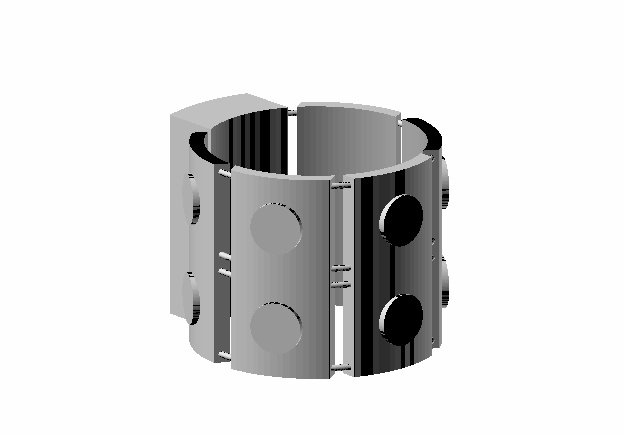
\includegraphics[width=0.45\textwidth]{graphics/bracelet-02.png}
%caption{Bracelet design with 2x5 tactor array.}
\end{center}
\end{figure}
\normalsize \color{red}
\begin{center}
\textbf{Bracelet design with 2x5 tactor array.}
\end{center}
\par

    \end{minipage}
    };
    \end{tikzpicture}
    \end{center}

%\begin{figure}[H]
%    \begin{center}
%        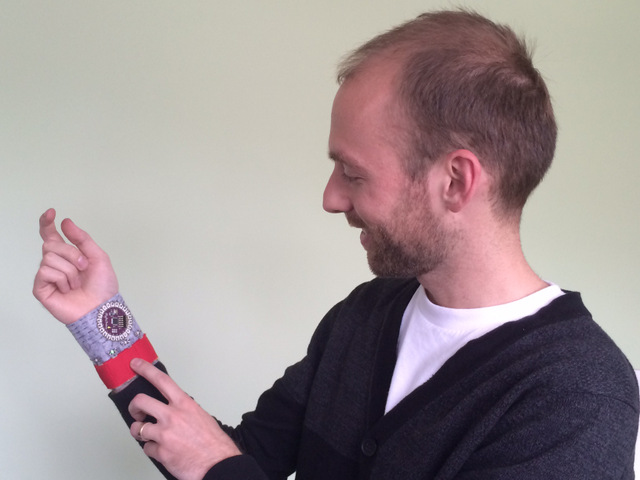
\includegraphics[width=0.4\textwidth]{graphics/hudsonBand.png}
%    \end{center}
%    \caption{A user playing a vibrotactile \textit{Simon Says} game on an earlier prototype. \label{fig:braceletRendering}}
%\end{figure}
%The design of vibe patterns for such devices is a specialized, yet multi-disciplinary domain that straddles concerns for design of human computer interfaces suitable for wearables, and for potentially artistic patterns that look and feel attractive on the wrist.

%coloured box with text
%\tikzstyle{mybox} = [draw=black, fill=orange!20, thick,
   % rectangle, rounded corners, inner sep=1cm, inner ysep=1cm]
\begin{center}
\begin{tikzpicture}
\node [textBox] (box) {
\begin{minipage}{0.45\textwidth}

\normalsize \color{black}
\textbf{Use cases for wrist-wearable device}
\begin{enumerate}
  \item Interpret wrist gestures and recognize overall physical activity of the wearer (using the microcontroller's accelerometer),
  \item notify the wearer when crystals and treasures are earned,
  \item offer vibrotactile clues about where crystals and treasures can be found, and
  \item provide aesthetically attractive and evocative vibe and light displays corresponding to narrative points in a story.
\end{enumerate}

\end{minipage}};
\end{tikzpicture}
\end{center}
    
%TEST BOX TEMPLATE vvvvvvvvvvvvvv
\begin{center}
\begin{tikzpicture}
\node [textBox] (box){ % or figureBox
\begin{minipage}{0.45\textwidth}
    
%Content goes here:
TEXT BOX TEMPLATE
    
\end{minipage}};
\end{tikzpicture}
\end{center}
%TEST BOX TEMPLATE ^^^^^^^^^^^^^^

    
It is use case no. 3 that we consider for its potential musicality and the applicability of musical-inspired pattern design. These patterns must be suitable for low resolution vibrotactile arrays -- in our case a 2x5 circular array of vibe motors, or \textit{tactors}, that encircle the wrist (Figure ~\ref{fig:braceletRendering}). 

%Concepts and entities expressed using standard musical notation such as notes, note durations, parts and instruments need to translated, or mapped, from the music domain to that of vibrotactile devices. This mapping has proven to be useful and appears to lead to interesting possibilities for pattern design for these devices.

%%%%%%%%%%%%%%%%%%%%%%%%%%%%%%%%%%%%%%%
\Huge \color{red}
\textbf{Research Problems}
\normalsize \color{black}
%%%%%%%%%%%%%%%%%%%%%%%%%%%%%%%%%%%%%%%

\normalsize \color{red}
\textbf{Haptic feedback and communication}\\
\normalsize \color{black}
The largest organ of the human body is the skin and has great potential for the transmittal of information and sensation.

% \cite{lindeman2006wearable} \cite{brewster2004tactons}. 

%Haptic communication through force feedback is a common technique used in gaming. Its purpose is to introduce the sense of touch to interactions such as movement through space, collision with objects, notification of awarding of game points and of proximity to dangerous situations. 

%Touch can add sensual aspects and realism to computer interactions for devices too small to have large visual displays and may be useful in reducing sensory overloads from other perceptual modalities such as those used in complex graphical interfaces \cite{oakley2000putting}. 

%Oakley provides a useful taxonomy of haptic-related terms, such as proprioceptive, kinesthetic and tactile. Haptic is a general term relating to the sense of touch, while tactile is more specific and relates to the sensation of pressure rather than that of temperature or pain \cite{oakley2000putting}. Haptic feedback has a long history in the design of computer mice and of other hand controllers \cite{yang2005novel}. Of course, 

%Touch can also be used to coordinate action between online collaborators and gamers by facilitating a sense of togetherness.

%\cite{ho1998experiment}.

touch is useful in generating intimacy in normal social situations. 

%\cite{bronner1982haptic}. 

%For example, the new Apple Watch enables wearers to communicate their heartbeat to others wirelessly.
%\cite{marks2014pulse}.\\ 

\normalsize \color{red}
\textbf{Wearable vibrotactile devices}\\
\normalsize \color{black}
%Typically, haptic devices beyond experimental contexts are either wearable or holdable. One challenge of wearable devices is motivating people to wear them. People tend to be very particular about the look and feel of devices that provide potentially intimate notifications. The purposes of such devices are varied and include emulation of attention-getting practices such as the squeezing of wrists, touching of shoulders and pats on arms. As Baumann notes, such social gestures may include a wealth of sub-texts including urgency, affection, control of the other and reinforcement of social hierarchies \cite{baumann2010emulating}. Due to their potential back or side-channel nature, vibrotactile devices could aid in tasks in which the user's main attention might be devoted to some other task, such as navigation, gameplay, or in situations where visual information is scarce or non-existent, as with the blind \cite{ertan1998wearable}.  Devices vary in the degree of body contact they provide. The ability of he body to perceiver vibrotactile stimuli varies greatly between regions of the body dues to variation in skin receptor density \cite{lindeman2006wearable}. Work has been also done in wide-area stimulation instead of areas of the body where receptor density is greatest, such as the tips of the fingers and lips \cite{lindeman2004towards}. Vibrational patterns suitable for a wrist device are much less complex than those designed for auditory perception due to the constrained perceptual channel of the cutaneous and kinaesthetic possibilities of the wrist compared to that of our ears.\\  

\normalsize \color{red}
\textbf{Tactile authoring for vibrotactile devices}\\
\normalsize \color{black}
%Wearable tactile devices are increasing in popularity, especially for handsfree applications. Tools for authoring of tactile patterns for these devices makes the job much easier. Pan�els, et al. describe a system for easy prototyping of tactile patterns based on a graphic representation of the shape of the device. A vibrotactile editor represents vibration pitch by vertical placement of notes, as in music notation. They describe the difficulty in designing such patterns by non-experts since it pre-supposes knowledge of music notation as well as other technical area like waveform design. Nor does the system support tactile design for multiple actuators \cite{paneels2013tactiped}. Brown examines how musical techniques can be applied to \textit{tacton} design. Tactons are structured vibrotactile messages designed to communicate information non-visually. They are the tactile counterpart of visual icons \cite{brewster2004tactons}. She examines the role of tactile dynamics and concludes that they should be combined with consideration of other vibrotactile parameters such as duration, roughness and rhythm \cite{brown2006tactile}. Gunther explores the notion of tactile composition, which he views as a novel coupling of haptics technology and music, for the purpose of creating aesthetically appealing tactile compositions. He notes the close relation between sound and touch in all musical performance. He later describes the complex psychophysics that informs the composition of spatio-temporal patterns on the skin  \cite{gunther2003cutaneous}.\\

\normalsize \color{red}
\textbf{Multiple actuator devices}\\
\normalsize \color{black}
%Devices that contain several vibrotactile actuators are common in the literature\cite{gunther2003cutaneous} \cite{lindeman2004towards} \cite{lindeman2006wearable} \cite{ertan1998wearable} \cite{brown2007tactons}. These devices tend to be placed at various locations around the body, or in tiny pin arrays suitable for fingertip stimulation \cite{brewster2004tactons}. The design of tactile patterns depends on the configuration and placement of the actuators. The purpose of having multiple actuators is distribute notifications of events in places around the body that will be noticed while people do other physically or cognitively demanding activities \cite{lindeman2006wearable}, to transmit symbolic information similar to the fingertip sensing of braille \cite{brewster2004tactons}, to develop skills with polyphonic rhythms  \cite{holland2010feeling}, providing feedback for digital musical instruments \cite{marshall2006vibrotactile} \cite{schumacher2013vibrotactile}, or to create aesthetically appealing patterns for the skin \cite{gunther2003cutaneous}. A wrist-worn bracelet similar to our device is described in \cite{paneels2013tactiped}.\\


\normalsize \color{red}
\textbf{Designing patterns using music notation}\\
\normalsize \color{black}
%\Huge \color{red}
%Introduction\\
%\normalsize \color{black}
%This research employs the text-based music engraving and compositional tool Lilypond \cite{nienhuys2003lilypond}. The application Frescobaldi [http://frescobaldi.org] was used as a front-end to Lilypond. Writing music using Lilypond is a similar process to writing papers using the document preparation system LaTex. Like LaTex, its textual input can be easily version-controlled. The output of Lilypond follows music notation conventions and is of high quality. Once learned to a rudimentary level Lilypond is a useful tool for experimenting with music notation and can easily output MIDI code. This MIDI is used to drive the actuator array in the vibrotactile bracelet using the standard Arduino MIDI library. The complete workflow is to first compose music in Frescobaldi/Lilypond, output a MIDI file from the Lilypond source, import this MIDI file into a track in Ableton Live, send a MIDI stream out from Ableton into a dedicated USB MIDI cable and then read this MIDI data in Arduino, using MIDI-read() function. The workflow proved to be quite workable as an experimental technique.\\

\normalsize \color{red}
\textbf{Basic mapping conventions}\\
\normalsize \color{black}
Our notational approach for our wrist-wearable device is to follow music notation conventions and to see where these conventions lead us in the domain of vibrotactile devices:

\begin{itemize}
\item Represent time horizontally from left to right. Notes to the right occur later.
\item A note represents an activation of a component. A component can be of several types (vibe motor, LED, etc.). Place notes on normal, five line staves.
\item Represent note durations by note type (for example, quarter, half and whole notes), dots and by ties between notes of the same pitch.
\item If notes are pitched, indicate their pitch through their vertical placement on a staff. If notes are unpitched, represent different components (e.g. different types of vibe motors or LEDs) using various note heads or annotations.
\item Different \textit{parts} are on separate staves. One tactor type playing the same notes at the same time represents playing in \textit{unison}. For example, eight vibe motors playing in unison can be represented as one part.
\item Simultaneous notes, or \textit{chords}, are stacked vertically as in music notation.
\end{itemize}

We also need to translate the nomenclature from the domain of wrist wearables to that of music notation. This mapping is shown in the following table:



\begin{center}
\begin{tikzpicture}
\node [textBox] (box){ % or figureBox
\begin{minipage}{0.45\textwidth}
    
\begin{table}[H]
\normalsize \color{black}\sffamily
%\caption{Vibrotactile vs Music notation terms}
\normalsize
%\centering
\begin{tabular}{@{}ll@{}}
%\toprule
\textbf{Vibrotactile term} & \textbf{Music notation term}\\ 
\midrule
Activation of one component & Note \\
Activation duration & Note duration \\
Frequency of an activation & Pitch \\
One type of component & Instrument \\
Series of activations for one component & Part \\
Simultaneous activations w/ multiple pitches & Chord \\
Integrated series of activations & Composition \\
%\bottomrule
\end{tabular}
\end{table}
    
\end{minipage}};
\end{tikzpicture}
\end{center}

%Therefore, the basic components of music are present even with a wrist-wearable vibrotactile device that does not, at first, seem to have a musical aspect: \textit{notes} with durations, pitched notes played on various discrete \textit{instruments} (vibe motors and LED lights), various \textit{parts,} or \textit{voices,} played in polyphonic \textit{compositions} and the dynamics of various parts playing together. \\

\normalsize \color{red}
\textbf{Pitch}\\
\normalsize \color{black}
%Vertical placement for normal, pitched notes in music notation indicates their pitch. Pitch differentials are possible with tactors, as their frequency can be modelled using standard pulse-width modulation (PWM) techniques \cite{lindeman2006wearable}. The pitch of a note is one of its primary psychoacoustic attributes, along with its duration, loudness and timbre. Unpitched notes are those for which the frequency is indeterminate, too complex or unrelated to the pitch contours of melodic or harmonic parts. The perception of pitch in vibrotactile devices differs from that of normal acoustic instruments. The number of frequency differences is much reduced and depends on amplitude. The skin's maximal frequency response occurs around 250 Hz \cite{gunther2003cutaneous}. There may be as few as five frequency distinctions possible with cutaneous perception, or as many as ten \cite{van2003distilling}.  So, the chromatic range of pitches and frequencies over many octaves as normally represented using music notation is not suitable for cutaneous perception, it appears that some, relatively minor variation in pitch is possible. These considerations would seem not to preclude the use of music notation for our purposes -- the use of notes to represent non-aural sensory expression.\\

\normalsize \color{red}
\textbf{Intensity}\\
\normalsize \color{black}
%The intensity of a vibrotactile stimulus is defined by the strength or magnitude of its vibration. As with aural music, suitable intensities for vibrotactile devices range from those that are barely perceptual to those that become uncomfortable. Classic work in this area was done by measuring Weber fractions and just noticeable differences (JNDs). Frequency and intensity parameters interact in vibrotactile studies in that differences can be ascribed to combinations of parameters \cite{van2003distilling}. The intensity threshold is adaptable and depends on a variety of parameters such as actuator used, location of the stimulation, person, or frequency of the vibration \cite{jonas2008tactile}. Geldard discovered that while we can discriminate 15 levels of vibrotactile stimuli intensity but that no more than three intensity levels can be identified absolutely \cite{geldard1960some}. Considerations of the amplitude envelope (amplitude, delay, sustain, release, or ADSR) and with amplitude modulations such as tremolo or pitch modulations like vibrato  are also important with vibrotactile stimulation \cite{gunther2003cutaneous}.\\

\normalsize \color{red}
\textbf{Duration}\\
\normalsize \color{black}
%The term duration refers to the length of the tactile stimulus -- from onset to the termination of the stimulus. There exist various reference values for duration and is generally measured in milliseconds \cite{jonas2008tactile}. It is important to ensure that the individual vibrotactile stimuli are within a reasonable range of durations. Geldard found that stimuli duration roughly between 0.1 and two seconds is reasonable \cite{geldard1960some}. If vibrotactile notes are of short duration they are perceived as sharp taps or jabs in the skin \cite{gunther2003cutaneous}, while stimuli that lasted longer than the upper limit of two seconds delays communication \cite{jonas2008tactile}. Dynamic properties of a vibration signal such as its envelope, duration, and the presence of masking stimuli may also affect perceptual threshold levels \cite{birnbaum2007musical}.\\

\normalsize \color{red}
\textbf{Spatial patterns and vibrotactile clues}\\
\normalsize \color{black}
%As noted above one of the primary use cases for our vibrotactile device is offer vibrotactile clues about where crystals and treasures can be found within transmedia-inspired gameplay. These clues are intended to provide the following messages to the game-player: \textit{Go this way / don't go that way}, and 
%\textit{You're getting warmer / you're getting colder}. These are spatial and metaphorical in nature and allude to navigating through some kind of virtual space. Pan�els discusses vibrotactile design for metaphorical patterns such as \textit{turn back} on devices that have actuators with spatial patterns, but does it in a non-musical context \cite{paneels2013tactiped}. Ideally these gameplay clues are either self-explanatory or easy for the player to learn. A vibrotactile device having a series of tactors activating in the intended direction might be a good first step in suggesting \textit{go this way}, much like a flashing series of traffic lights scrolling to the right suggest proceed to the right (Figure ~\ref{fig:tactorArray}). To test such intuitions requires additional study. One should also note that wrist-worn devices can be oriented in various ways, depending on wrist position.\\

%Music as it is commonly notated does not lend itself to these sorts of concepts or metaphors. Although music that has spatial aspects is common, such as the surround sound of Thomas Tallis' \textit{Spem in Alium} [1570], or the call and response of antiphonal works, standard music notation tends not to focus on the specification of spatial aspects in music performance -- even though aural perception is intensely spatial. In ensembles, sections of instruments playing the same parts are usually placed together but this is a performance convention and is usually outside of the notation itself. Therefore, it is unclear at first what notated music that could be interpreted as \textit{go this way}, or \textit{you're getting warmer} might look like.\\


\begin{figure}[H]
\definecolor{light-gray}{gray}{0.85}
\definecolor{med-gray}{gray}{0.65}
\definecolor{dark-gray}{gray}{0.35}
  	
	%\begin{tikzpicture}[scale=2.0]
	\begin{center}
	\begin{tikzpicture}[scale=2]
	%arrow on top:
	\draw[thick,->, line width=2pt] (0.5,2.5) -- (4.5,2.5);
	%curved arrows:
	%\draw[thick,->,>=angle 90, line width=2pt, shorten >=10pt, shorten <=10pt] 
		%(4.5,1.5) .. controls (9,3) and (-4,3) .. (0.5,1.5);
	%\draw[thick,->,>=angle 90, line width=2pt, shorten >=10pt, shorten <=10pt] 
		%(4.5,0.5) .. controls (9,-1) and (-4,-1) .. (0.5,0.5);
	%grid:
	\draw[step=1cm,gray,very thin] (0,0) grid (5,2);
	%bottom row:
	\filldraw[fill=dark-gray, draw=black] (0.5,0.5) circle (0.12cm);
	\filldraw[fill=white, draw=black] (1.5,0.5) circle (0.12cm);
	\filldraw[fill=white, draw=black] (2.5,0.5) circle (0.12cm);
	\filldraw[fill=white, draw=black] (3.5,0.5) circle (0.12cm);
	\filldraw[fill=white, draw=black] (4.5,0.5) circle (0.12cm);
	%top row:
	\filldraw[fill=dark-gray, draw=black] (0.5,1.5) circle (0.12cm);
	\filldraw[fill=white, draw=black] (1.5,1.5) circle (0.12cm);
	\filldraw[fill=white, draw=black] (2.5,1.5) circle (0.12cm);
	\filldraw[fill=white, draw=black] (3.5,1.5) circle (0.12cm);
	\filldraw[fill=white, draw=black] (4.5,1.5) circle (0.12cm);

	\end{tikzpicture}
	\end{center}
  	%\caption{2x5 array of tactors with directional activation.}
  	\label{fig:tactorArray}

\end{figure}
\begin{center}
\textbf{2x5 array of tactors with directional activation.}
\end{center}

\bigskip
\bigskip

%vvvvvvvvv%%%%%%%%%%%%%%%%%%%%%%%%%%%%%%%%%%
%http://tex.stackexchange.com/questions/18363/diagrams-package-that-allows-to-draw-computer-buffers-memory-diagrams

%\begin{center}
%\begin{tikzpicture}[>=latex,font=\sffamily,semithick,scale=3]
%    \fill [green!25] (0,0) -- (67.5:1) arc [end angle=-22.5, start angle=67.5, radius=1] -- cycle;
%    \draw [thick] (0,0) circle (1);
%    \foreach \angle in {90,67.5,...,-67.5}
%        \draw (\angle:1) -- (\angle-180:1);
%    \node [circle,thick,fill=white,draw=black,align=center,minimum size=3cm] at (0,0) {FIFO as a\\Circular Buffer};
%    \draw [<-] (56.25:1) -- (56.25:1.25) -- +(.333,0)
%        node [right,inner xsep=.333cm] (Head) {Head (extract)};
%    \draw [<-] (-33.75:1) -- (-33.75:1.25) -- +(.333,0)
%        node [right,inner xsep=.333cm] (Tail) {Tail (insert)};
%    \draw [->,shorten >=5pt,shorten <=5pt] (Tail.west) to [bend right] 
%        node [midway,sloped,above,allow upside down] {\footnotesize 4\,bytes in FIFO}
%    (Head.west);
%\end{tikzpicture}
%\par
%\textbf{Circular array 1}
%\end{center}

\begin{center}
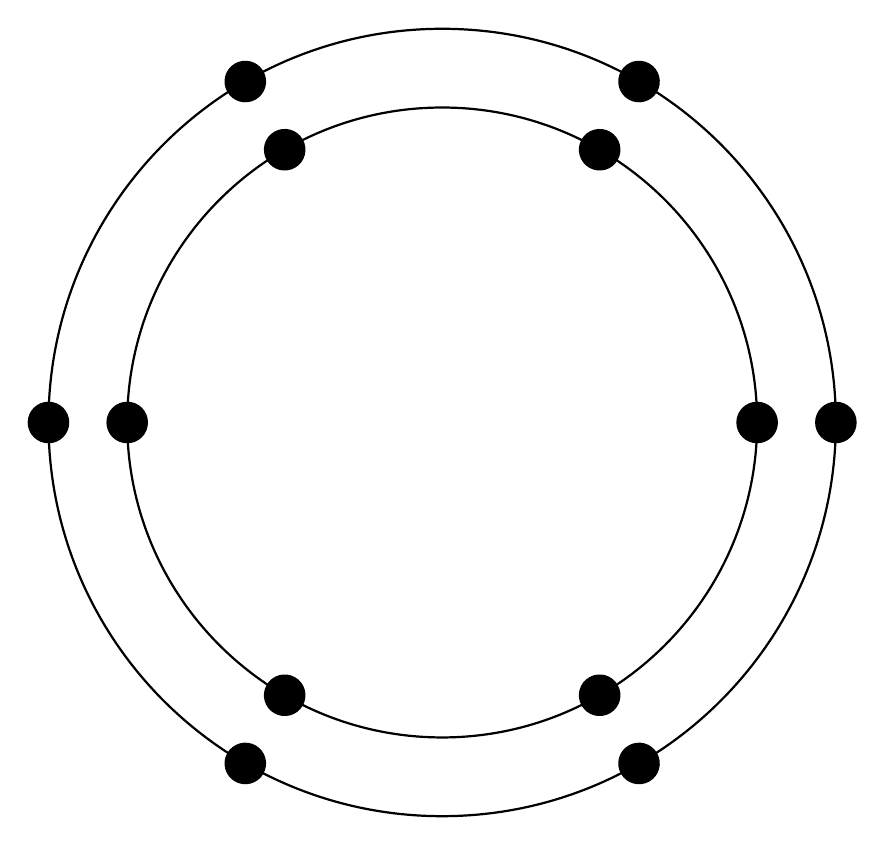
\begin{tikzpicture}
\draw [thick] (0,0) circle (4);
\draw [thick] (0,0) circle (5);
\foreach \angle in {0,60,...,300}
	\draw [thick, fill=black, rotate=\angle, shift={(5, 0)}] (0,0) circle (0.25);
\foreach \angle in {0,60,...,300}
	\draw [thick, fill=black, rotate=\angle, shift={(4, 0)}] (0,0) circle (0.25);
\end{tikzpicture}
\par
\textbf{Circular array of tactors.}
\end{center}

\bigskip
\bigskip


\par
\bigskip
\begin{center}
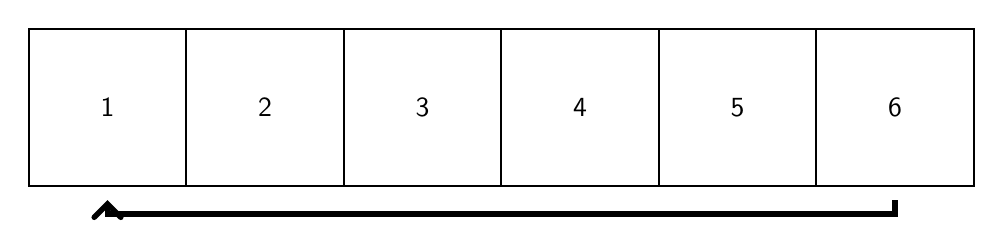
\begin{tikzpicture}[>=latex,font=\sffamily,every node/.style={minimum width=2cm, minimum height=2cm, outer sep=0pt, draw=black, thick}]
        \node at (0,0) (A) {1};
        \node [anchor=west] at (A.east) (B) {2};
        %\draw [anchor=west] at (A.east) circle (0.25);
        \node [anchor=west] at (B.east) (C) {3};
        \node [anchor=west] at (C.east) (D) {4};
        \node [anchor=west] at (D.east) (E) {5};
        \node [anchor=west] at (E.east) (F) {6};
        \draw [thick,->,>=angle 90, line width=2pt, shorten >=5pt, shorten <=5pt] 			(F.south) -- +(0,-1em) -| (A);
\end{tikzpicture}
\par
\textbf{Linear array of tactors.}
\end{center}
\bigskip
\bigskip
%^^^^^^^^^%%%%%%%%%%%%%%%%%%%%%%%%%%%%%%%%%


%%%%%%%%%%%%%%%%%%%%%%%%%%%%%%%%%%%%%%%
\Huge \color{red}
\textbf{Controlling Components\\ using Musical Notation\\}
\normalsize \color{black}
%%%%%%%%%%%%%%%%%%%%%%%%%%%%%%%%%%%%%%%

\normalsize \color{red}
%\textbf{Music with one spatial dimension (1D = linear)}\\
\normalsize \color{black}
%Following this line of reasoning, music with one spatial dimension is that which instruments follow some kind of spatial linear progression along one line, such as pan or a sweep. Figure ~\ref{fig:arrowsMoving00}. shows one vibe motor activating in a simple rhythm with a simple, rhythmic pitch change. 
%By the conventions of music notation it is clear that a regular rhythm is being represented. Of course, to appreciate this requires at least a rudimentary knowledge of music notation. To design a pattern of similar rhythmic complexity by means other than music notation would likely be more difficult. \\

%ZERO DIM
\begin{center}
\begin{tikzpicture}
\node [figureBox] (box){ % or figureBox
\begin{minipage}{0.45\textwidth}
\begin{center}
\Large \color{red} \textbf{Device with no spatial dimension (0D = point)}\\
\textbf{Vertical note position maps to single component}\\
\normalsize
\color{black}
\vspace{2cm}
%top diagram
\begin{tikzpicture}[scale=2]
%grid
\draw[step=1cm,gray,very thin] (0,0) grid (1,1);
%circles:
\filldraw[fill=blue, draw=black] (0.5,0.5) circle (0.12cm);
%\draw[very thin] (0.5,0.5) circle (0.2cm);
%\draw[very thin] (0.5,0.5) circle (0.35cm);

\end{tikzpicture}\\
\textbf{Device with a single vibe motor}
\vspace{1cm}
%bottom figure (musical staff)
\begin{figure}[H]
        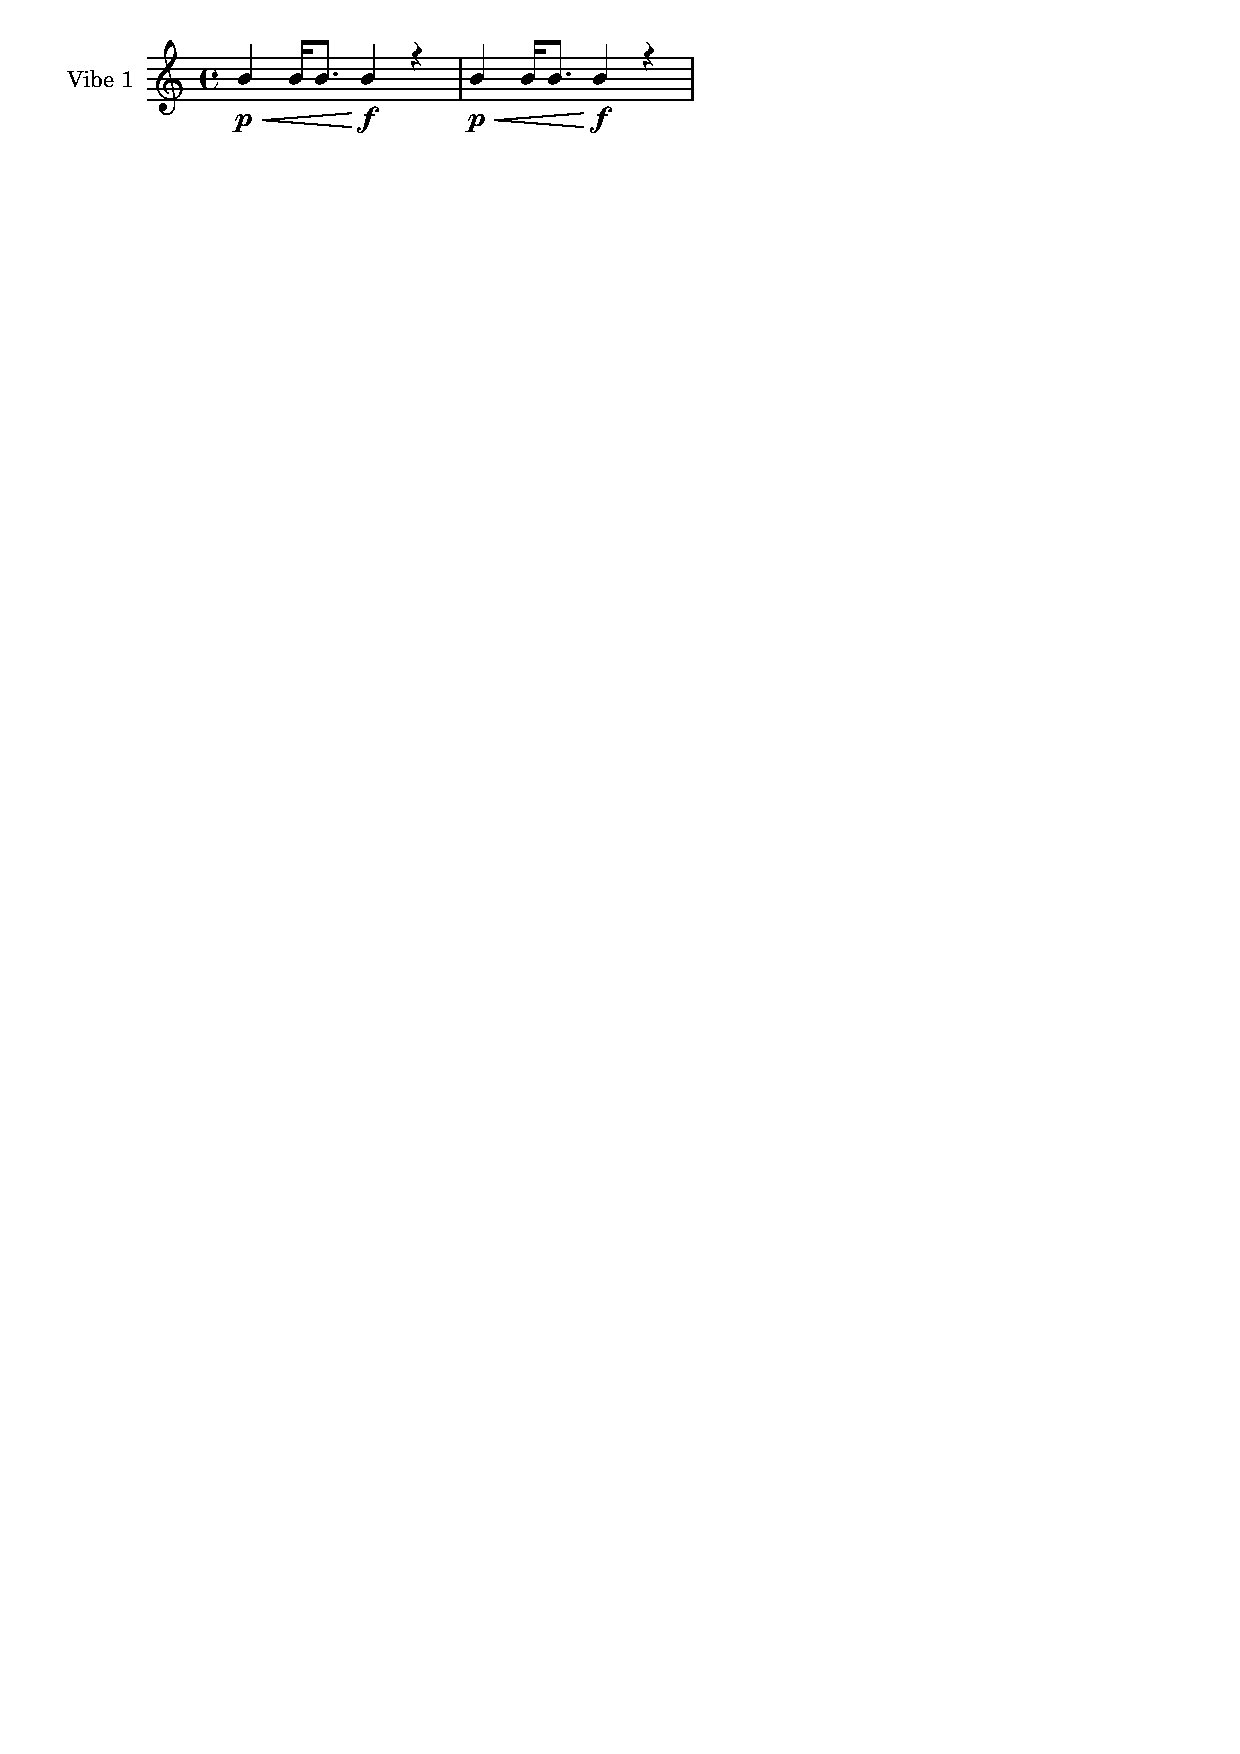
\includegraphics[width=0.65\textwidth]{graphicsPoster/arrowsMoving-00.pdf}
\end{figure}
\textbf{Score for single vibe motor playing a simple solo rhythm}\\
\begin{itemize}
\item Specifies activation for a single component
\item Time = horizontal axis. Horizontal, or rhythmic information as per standard musical notation
\item Vertical position does not vary (therefore, unpitched notation would also be suitable)
\item For most vibe motors pitch remains constant, but intensity can vary
\item Intensity specified by dynamics markings
\item Information is not very dense (single line score would suffice)
\item \textbf{NEXT STEP} notate for multiple vibe motors
\end{itemize}
\end{center}
\end{minipage}};
\end{tikzpicture}
\end{center}

%ONE DIM, unpitched
\begin{center}
\begin{tikzpicture}
\node [figureBox] (box){ % or figureBox
\begin{minipage}{0.45\textwidth}
\begin{center}
\Large 
\color{red} \textbf{Device with one spatial dimension (1D = linear)}\\
\textbf{Vertical note position maps to five components}\\
\normalsize
\color{black}
\vspace{2cm}
%top diagram
\begin{tikzpicture}[scale=2]
%grid
\draw[step=1cm,gray,very thin] (0,0) grid (5,1);
%bottom row:
\filldraw[fill=blue, draw=black] (0.5,0.5) circle (0.12cm);
\filldraw[fill=white, draw=black] (1.5,0.5) circle (0.12cm);
\filldraw[fill=white, draw=black] (2.5,0.5) circle (0.12cm);
\filldraw[fill=blue, draw=black] (3.5,0.5) circle (0.12cm);
\filldraw[fill=white, draw=black] (4.5,0.5) circle (0.12cm);
\end{tikzpicture}\\
\textbf{Device with a line of vibe motors}.
\vspace{2cm}
%bottom figure (musical staff)
\begin{figure}[H]
        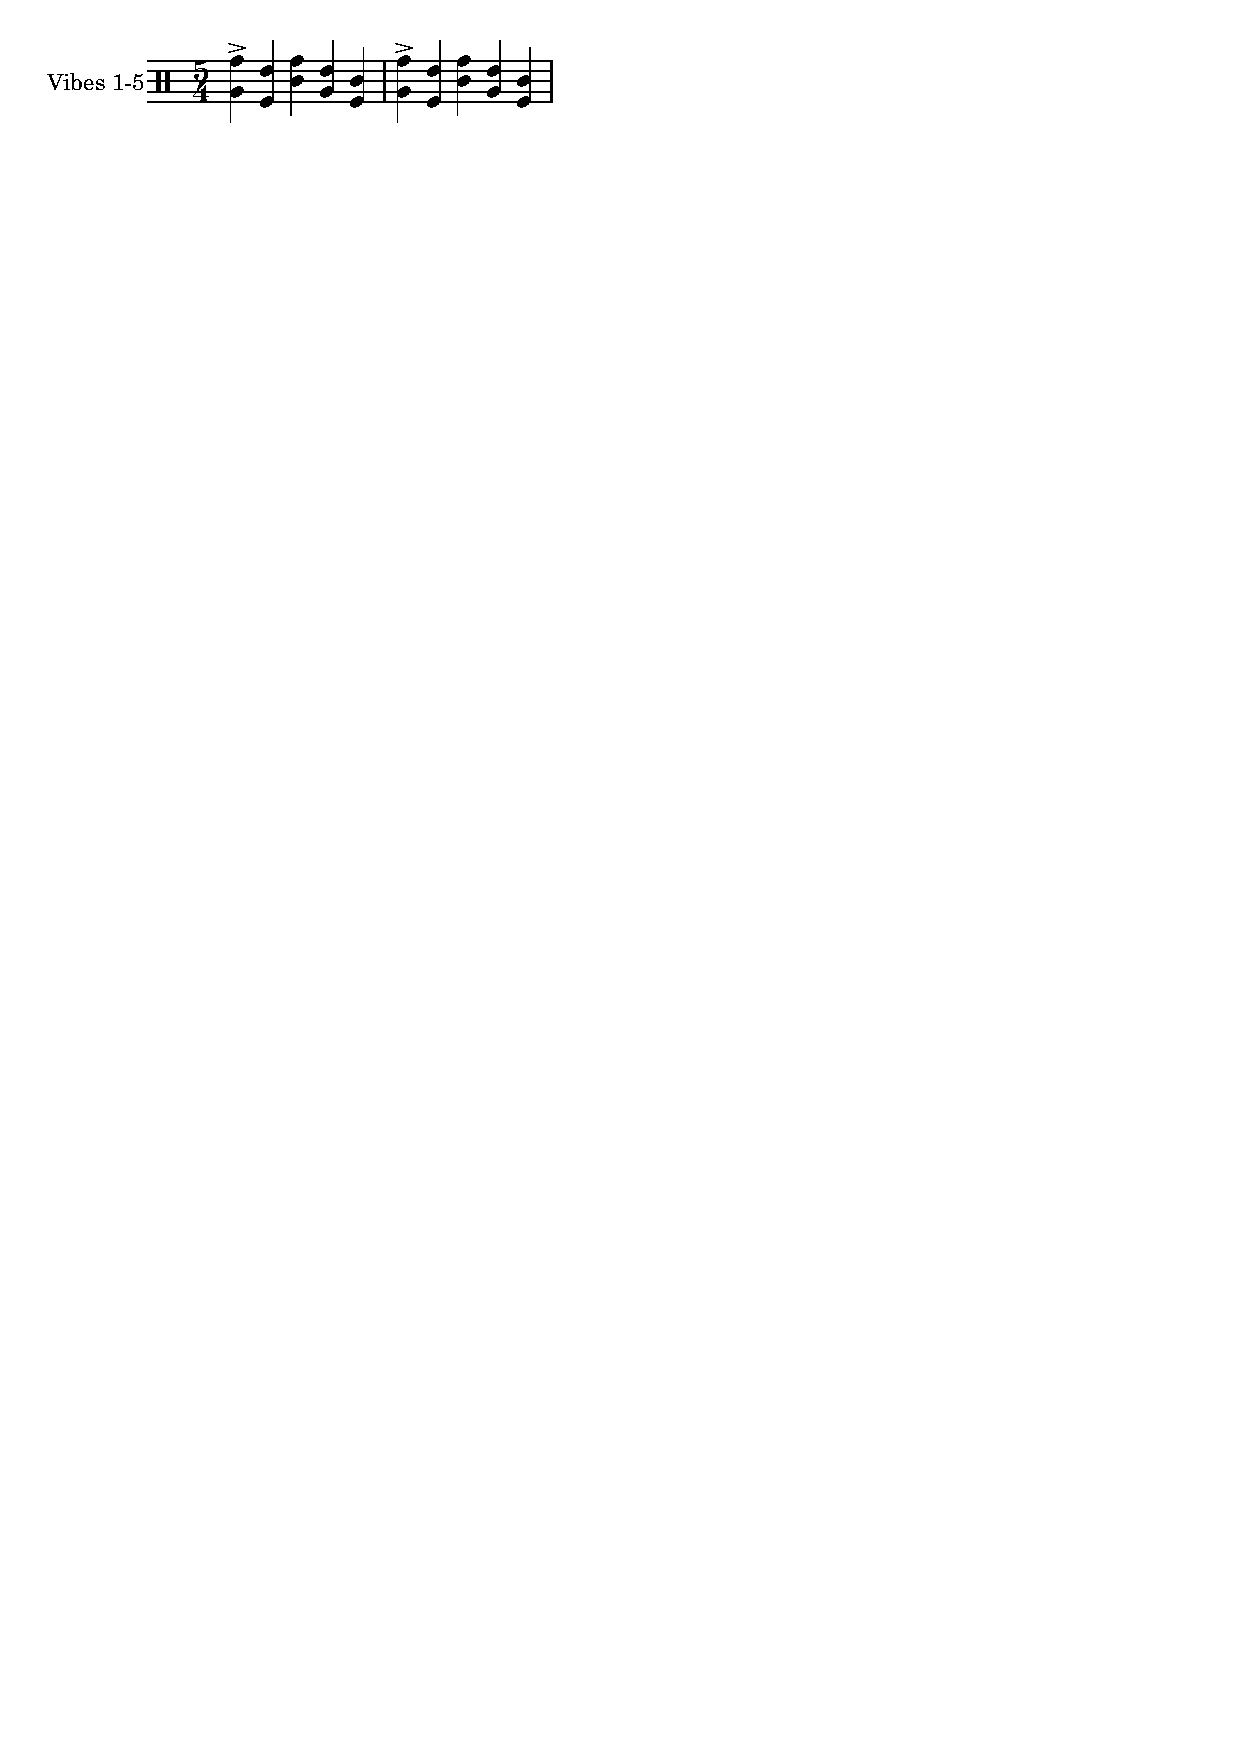
\includegraphics[width=0.85\textwidth]{graphicsPoster/arrowsMoving-00-drumStaff.pdf}
\end{figure}
\textbf{Score for a linear array of five vibe motors}
\begin{itemize}
\item Specifies activations for five, independent components
\item Time = horizontal axis
\item Notation is for unpitched components and has five lines
\item Each part occupies one staff line (rests are hidden)
\item Vertical staff position specifies vibe motor to activate; top line=1, second line=2, etc.
\item MIDI number for note $\Rightarrow$ vibe motor address
\item \textbf{PROBLEM} Putting five parts on one staff is hard to read 
\item \textbf{NEXT STEP} Make notation less dense and more readable
\end{itemize}

%ONE DIM, low density
\begin{center}
\vspace{2cm}
%bottom figure (musical staff)
\begin{figure}[H]
        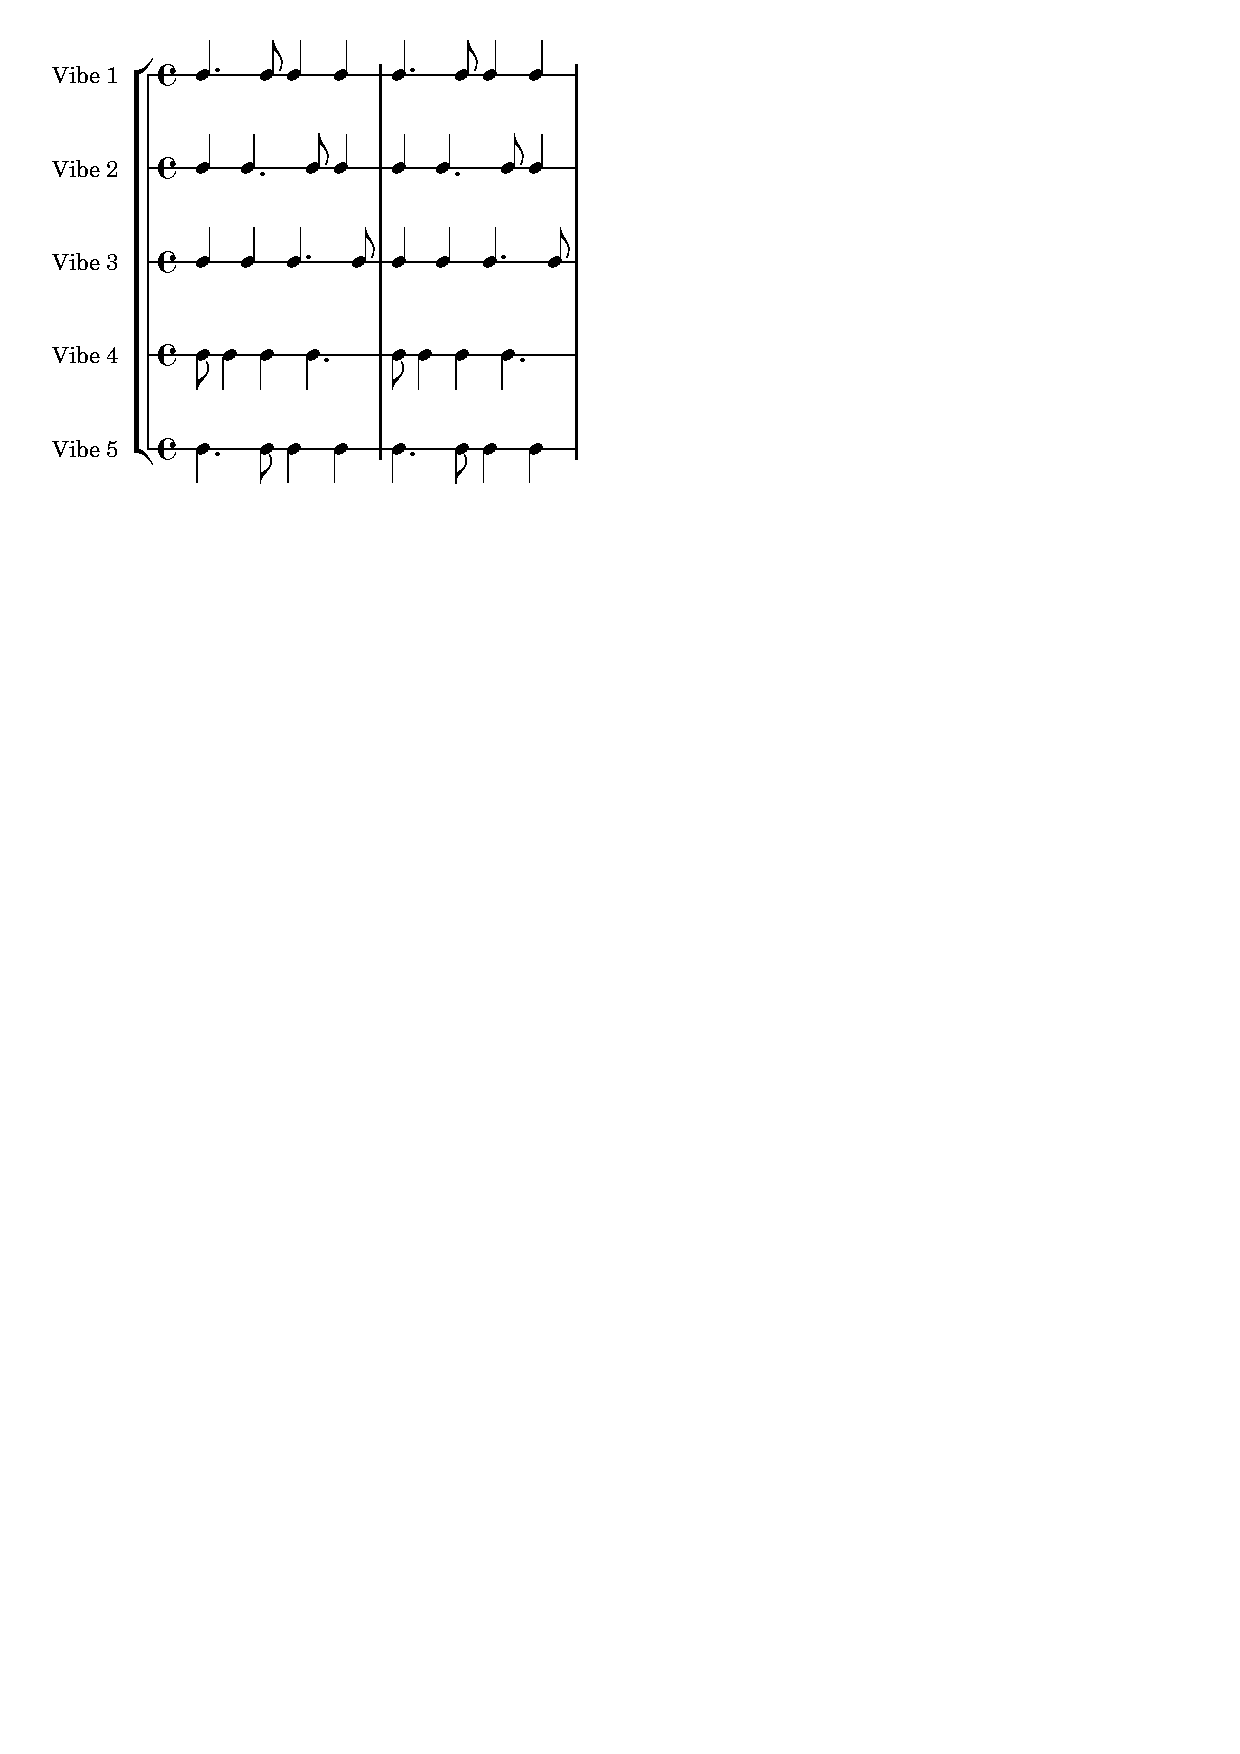
\includegraphics[width=0.65\textwidth, height=.35\textwidth]{graphicsPoster/arrowsMoving-01-drumStaves.pdf}
\end{figure}
\textbf{Score for a linear array of five vibe motors}
\begin{itemize}
\item Specifies activations for five, independent components
\item Time = horizontal axis
\item Five staff rhythmic notation 
\item MIDI number derived from staff $\Rightarrow$ vibe motor address
\item \textbf{NEXT STEP} Make notation suitable for two dimensional arrays of vibe motors
\end{itemize}
\end{center}
\end{center}
\end{minipage}};
\end{tikzpicture}
\end{center}


%TWO DIM
\begin{center}
\begin{tikzpicture}
\node [figureBox] (box){ % or figureBox
\begin{minipage}{0.45\textwidth}
\begin{center}
\Large
\color{red} \textbf{Device with two spatial dimension (2D = planar)}\\
\normalsize
\color{black}
\vspace{2cm}
%top diagram
\begin{tikzpicture}[scale=2]
%grid
\draw[step=1cm,gray,very thin] (0,0) grid (5,2);
%top row:
\filldraw[fill=white, draw=black] (0.5,1.5) circle (0.12cm);
\filldraw[fill=blue, draw=black] (1.5,1.5) circle (0.12cm);
\filldraw[fill=white, draw=black] (2.5,1.5) circle (0.12cm);
\filldraw[fill=white, draw=black] (3.5,1.5) circle (0.12cm);
\filldraw[fill=blue, draw=black] (4.5,1.5) circle (0.12cm);
%bottom row:
\filldraw[fill=blue, draw=black] (0.5,0.5) circle (0.12cm);
\filldraw[fill=white, draw=black] (1.5,0.5) circle (0.12cm);
\filldraw[fill=white, draw=black] (2.5,0.5) circle (0.12cm);
\filldraw[fill=blue, draw=black] (3.5,0.5) circle (0.12cm);
\filldraw[fill=white, draw=black] (4.5,0.5) circle (0.12cm);
\end{tikzpicture}\\


\textbf{Device with an array of vibe motors}
\vspace{2cm}
%bottom figure (musical staff)
\begin{figure}[H]
        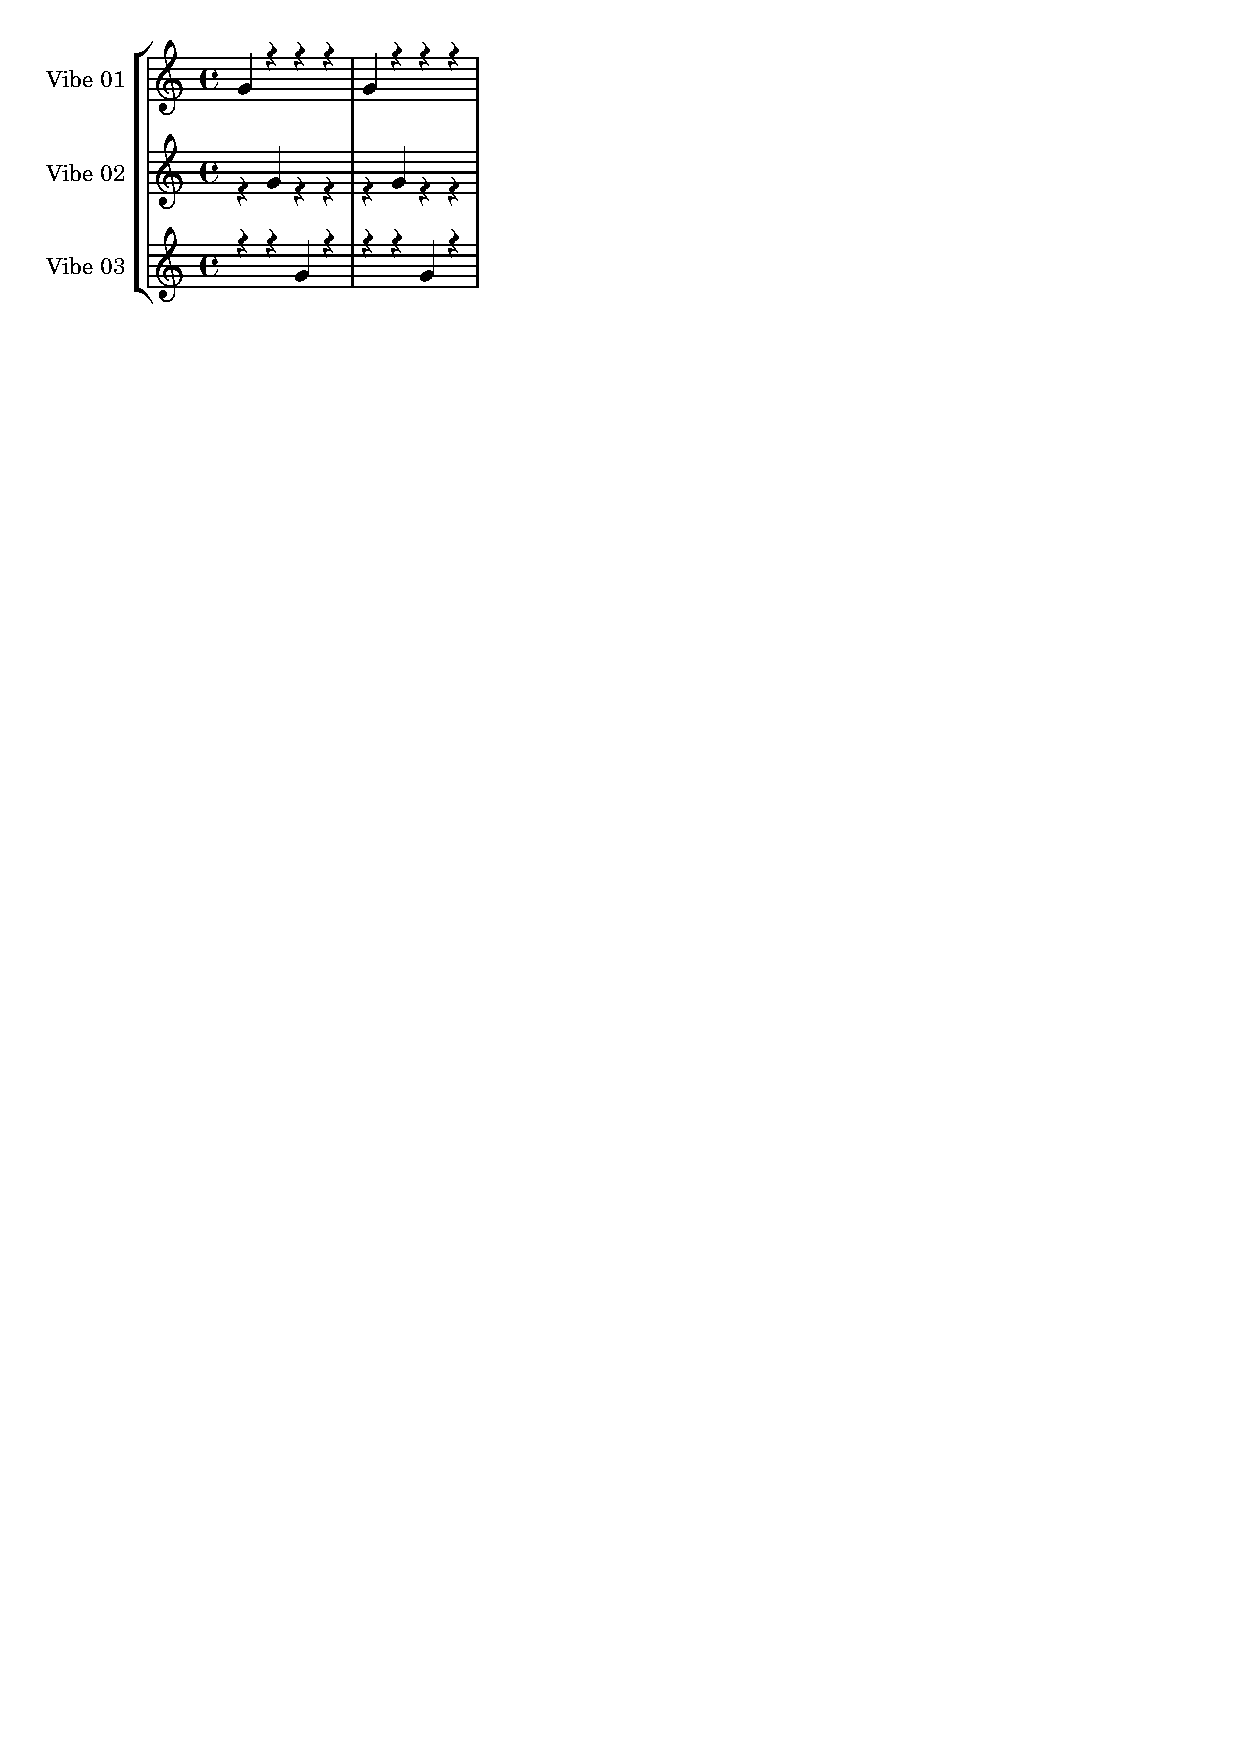
\includegraphics[width=0.75\textwidth]{graphics/arrowsMoving-01.pdf}
\end{figure}
\textbf{Score for an array of vibe motors}
\begin{itemize}
\item Time = horizontal, x-axis (rests are hidden)
\item Vertical staff position (EGBDF) = vibe motor address
\item Vertical position no longer signifies pitch
\item Separate part for each vibe motor
\item Each component is independently addressable through notation
\item Accents and other articulations possible
\end{itemize}
\end{center}
\end{minipage}};
\end{tikzpicture}
\end{center}


%\begin{figure}[htb]
%    \begin{center}
%        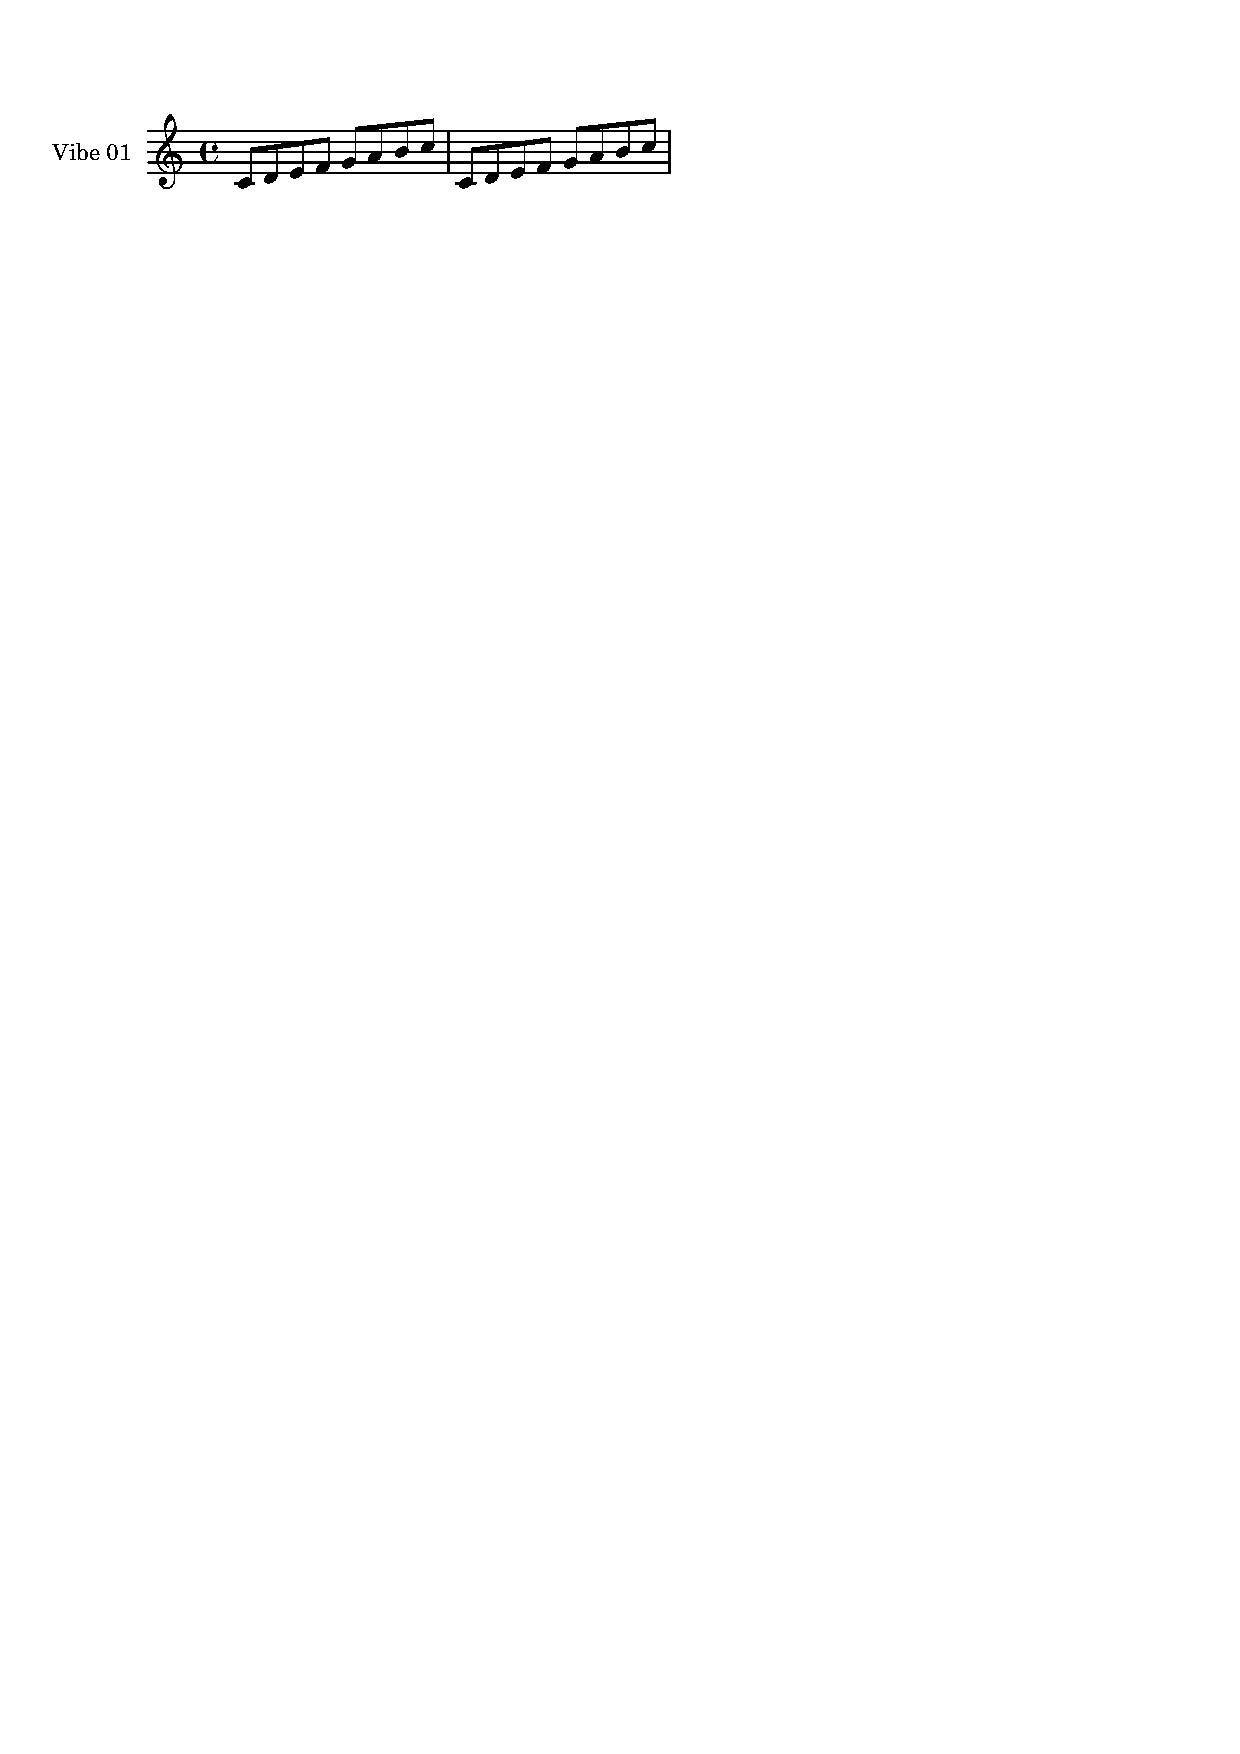
\includegraphics[width=0.4\textwidth]{graphics/scaleArduino-01.pdf}
%    \end{center}
%    \caption{Simple scale for a pitched Arduino component.\label{fig:fig2}}
%\end{figure}

%\begin{figure}[htb]
%    \begin{center}
%        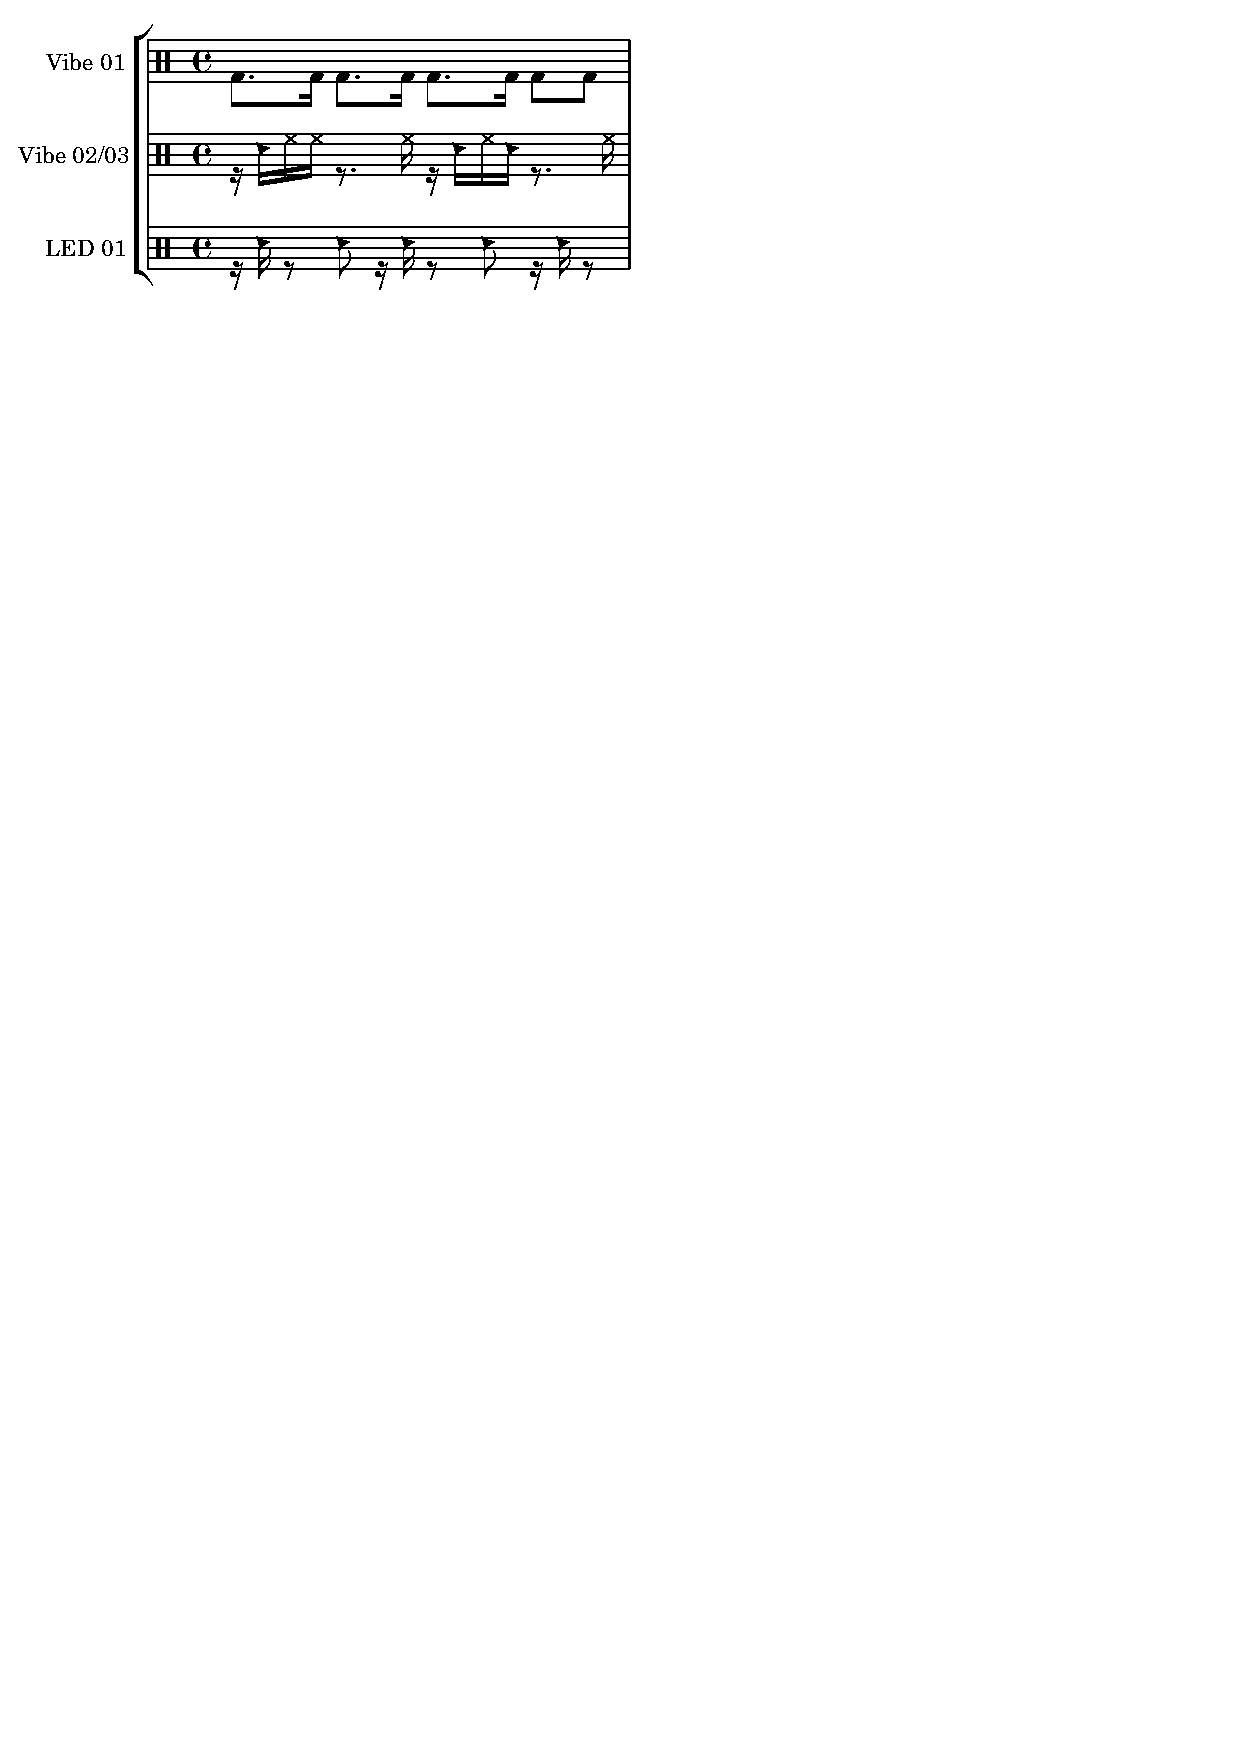
\includegraphics[width=0.4\textwidth]{graphics/drums1-multistaff.pdf}
%    \end{center}
%    \caption{Complex rhythm for three Arduino components.\label{fig:fig4}}
%\end{figure}

%\begin{figure}[htb]
%    \begin{center}
%        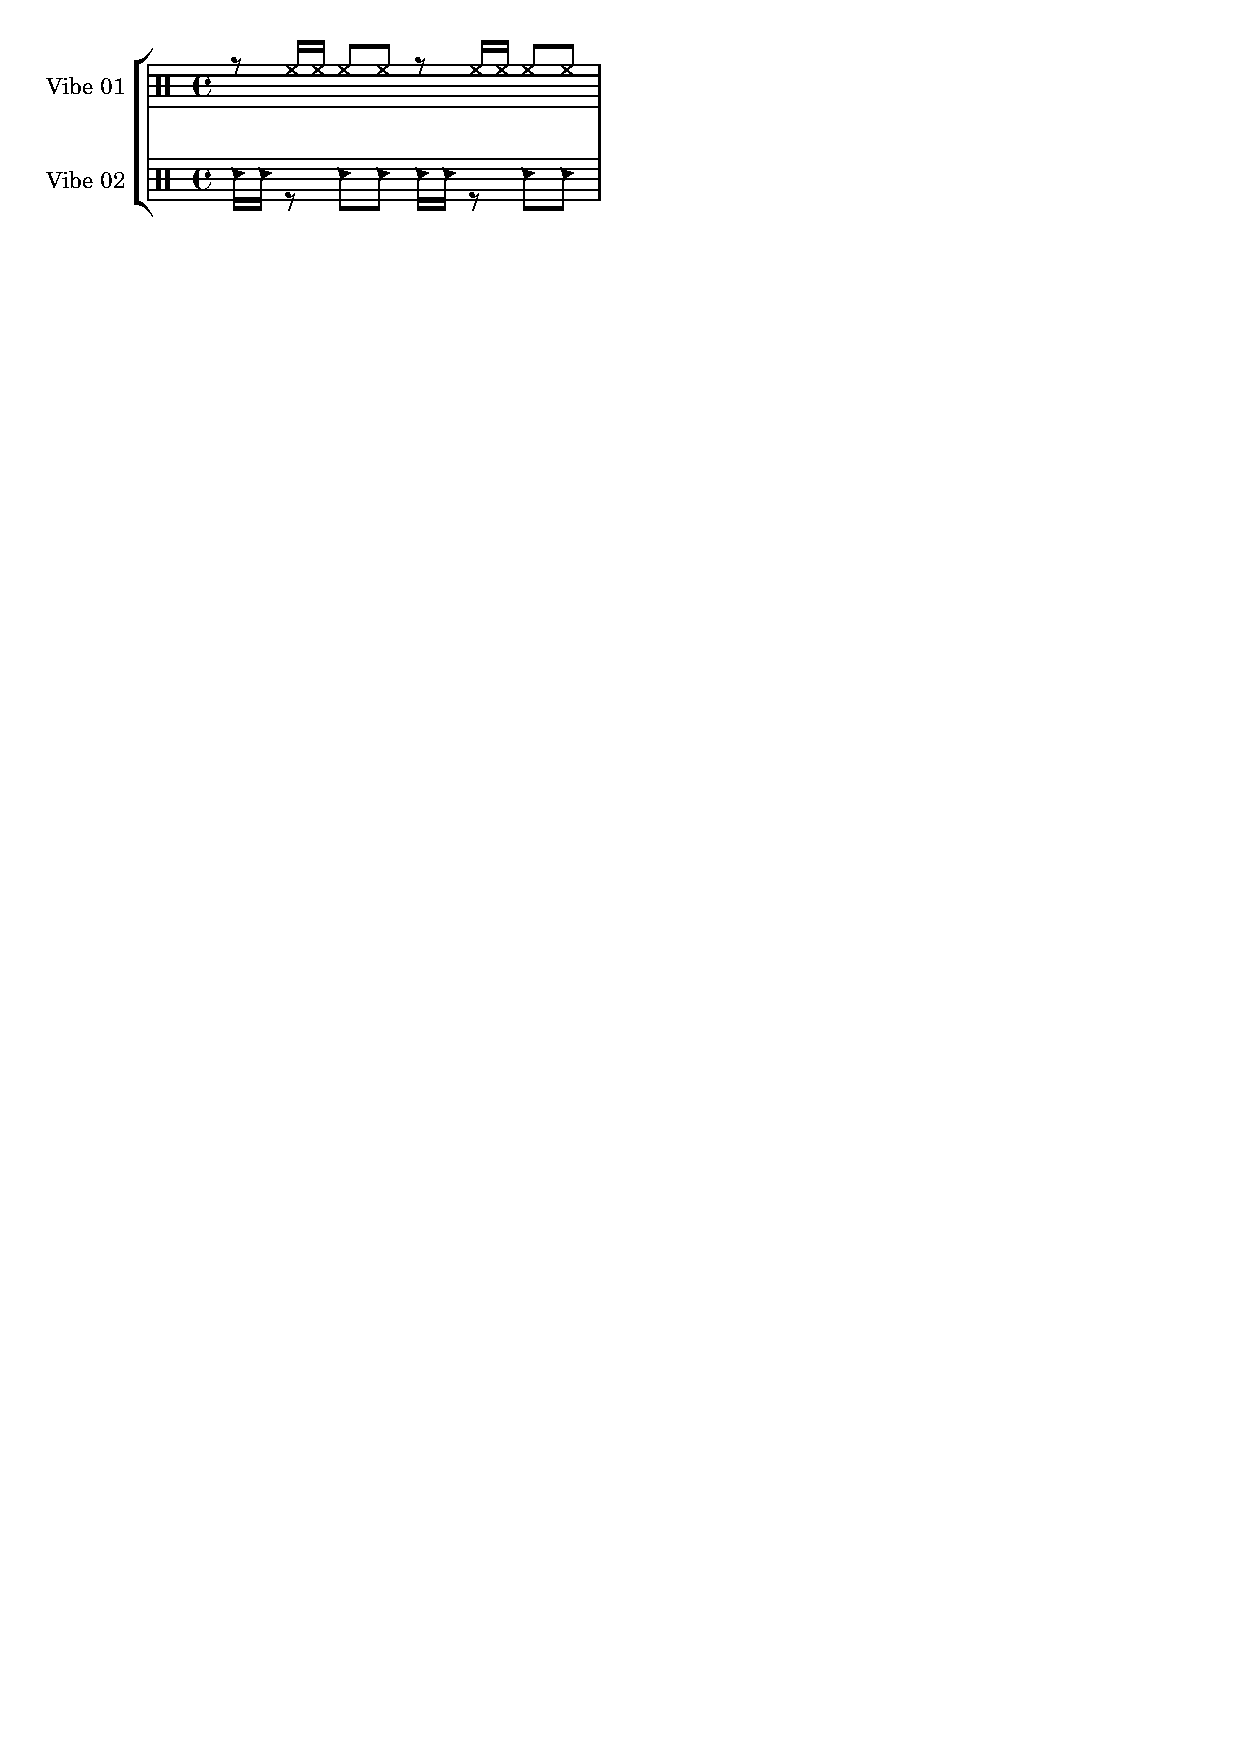
\includegraphics[width=0.3\textwidth]{graphics/drums1-simple.pdf}
%    \end{center}
%    \caption{Simple rhythm for two unpitched Arduino components.\label{fig:fig3}}
%\end{figure}

%\begin{figure}[H]
%    \begin{center}
%       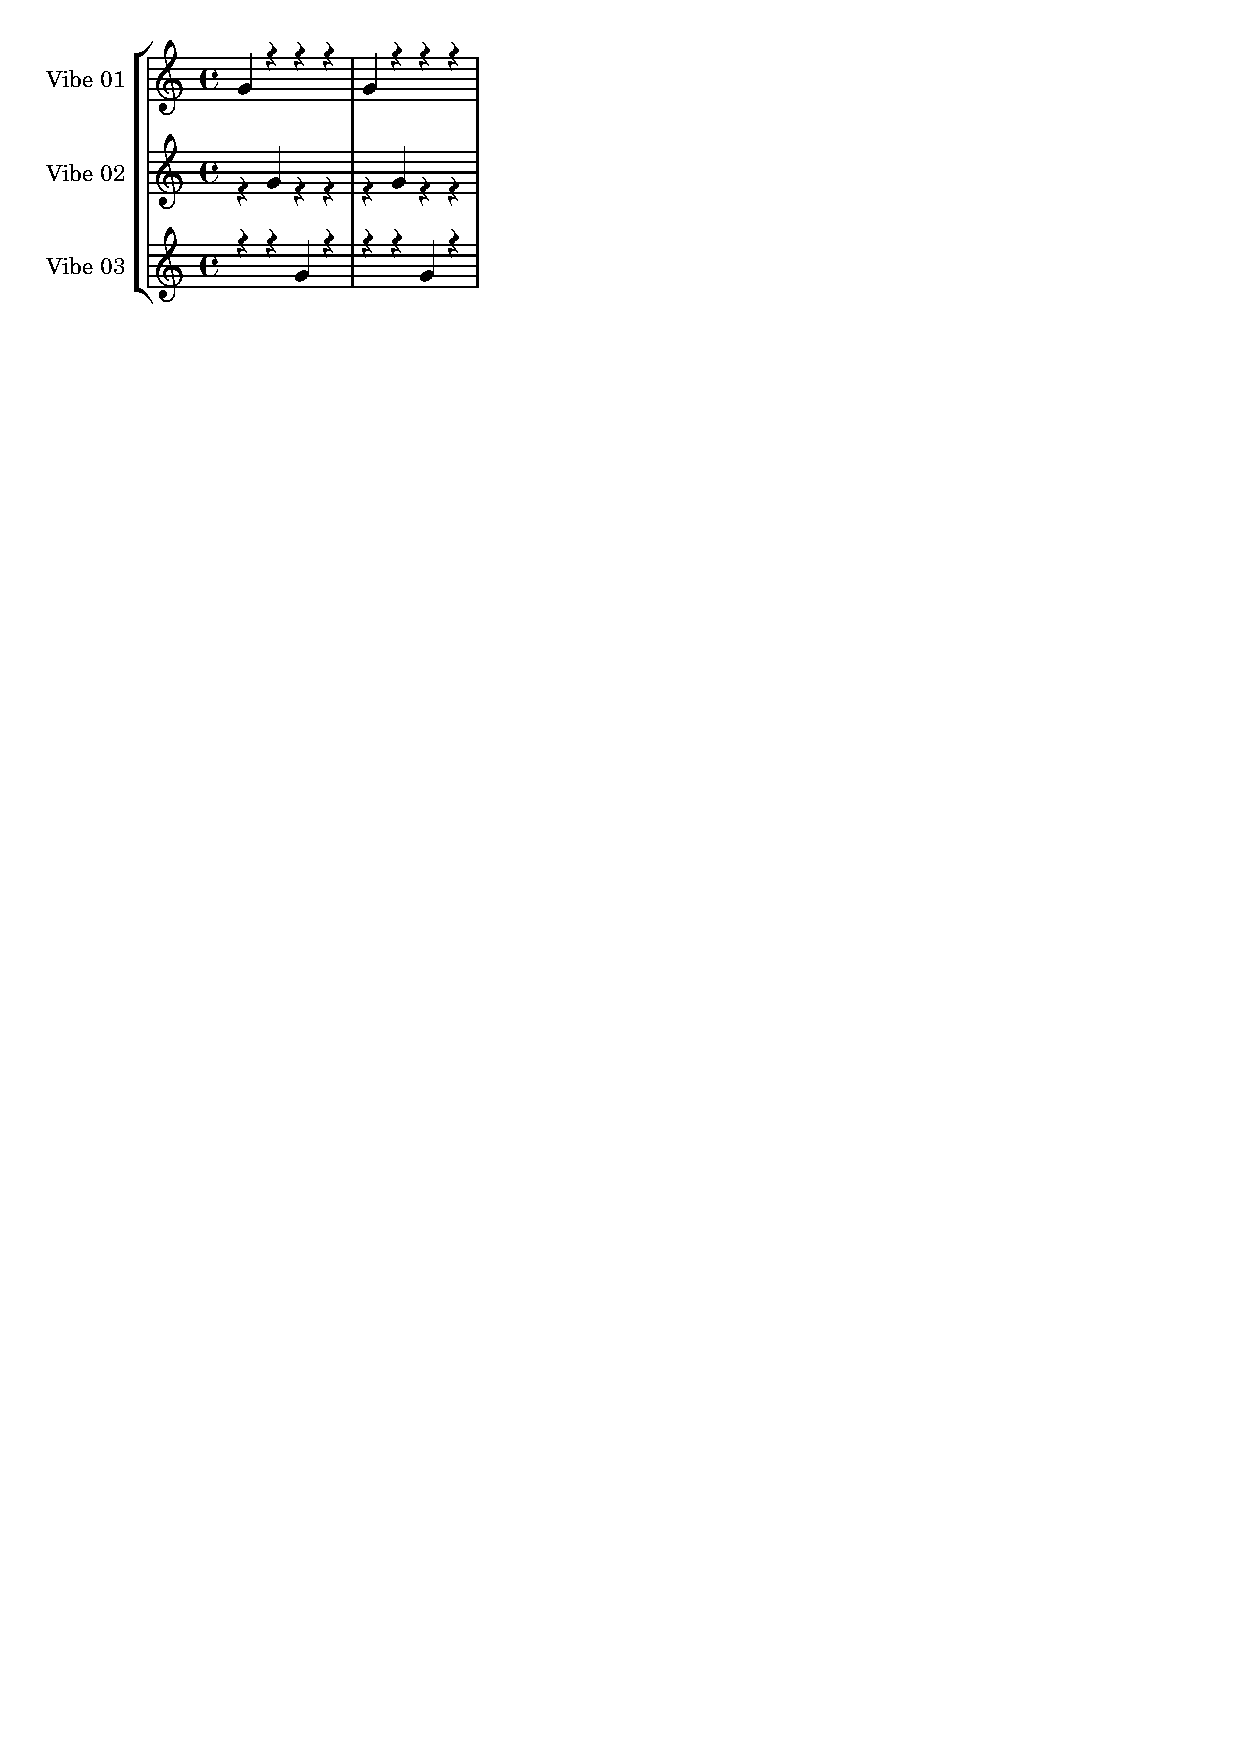
\includegraphics[width=0.3\textwidth]{graphics/arrowsMoving-01.pdf}
%  \end{center}
%  \caption{Threes vibes activating sequentially.\label{fig:arrowsMoving01}}
%\end{figure}

%Figure ~\ref{fig:arrowsMoving01}. shows three vibe motors activating in a sequential motion. The motors are arranged along a line and therefore are only one dimensional. Since they are playing the same pitch if the three separate parts where placed on the same staff there would be confusion about which note applies to which motor. Because of their linear placement their pulsation has a directionality. However, this directionality is less apparent in the notation itself. The only indication that Vibe 02 might be located after Vibe 01 is because of the numbering of the score. Yet with vibe bracelets it is desirable to be able to represent two dimensions such that common 2D patterns such as moving sprites, radiating waves and the like can be created across the skin. Is it possible to easily represent the activation of a 2D array of instruments using standard music notation?\\

\normalsize \color{red}
\textbf{Music with additional spatial dimensions (2D = planar)}\\
\normalsize \color{black}
%With pitched notation the pitch, timing and rhythm of the music tends to be its most important aspect. Time occupies the \textit{x} dimension while pitch occupies the \textit{y}. The spatial placement of the instruments playing different parts is less of a concern. You can have many \textit{parts}, or stack notes in \textit{chords} but this seems only to provide you with one additional dimension. With variables outside of standard notation, such as those that can be accessed though midi channels, additional mappable dimensions may be possible but then this becomes similar to using other programming techniques in which dimensions of information are represented using, for instance, multi-dimensional arrays. The clear graphic presentation of standard music notation, which could be so useful in depicting complex music patterns, would then be lost.\\

%\normalsize \color{red}
%Future Work\\
%\normalsize \color{black}
%Our work consists of quick iteration of devices and authoring of activation patterns for several devices. This work is motivated by both research and aesthetic considerations. Pattern authoring depends crucially on the nature of the device being authored for and its purpose. We consider two aspects that seem particularly promising for future development in this area: the design of vibrotactile patterns to enhance and inform transmedia narratives, and the creation of aesthetically appealing vibrotactile patterns in a variety of musical \textit{genres}. We are also interested in ways of packing more information into standard music notation since it provides a means of representing complex patterns of activation in an elegant form.\\

%%%%%%%%%%%%%%%%%%%%%%%%%%%%%%%%%%%%%%%
\Huge \color{red}
\textbf{Conclusion}
\normalsize \color{black}
%%%%%%%%%%%%%%%%%%%%%%%%%%%%%%%%%%%%%%%

%Music notation is a finely structured notational system. It requires an expert-level of competence to read its finest levels of detail, however, this type of expertise is not hard to find in cultures where notated musical composition and performance is well-established. What is much less common is cross-expertise in both music notation and vibrotactile technologies. Designing interesting and functionally useful patterns for vibrotactile devices is obviously a new field. Standard musical notation includes many dimensions but in its standard forms does not easily lend itself to inclusion of additional non-musical dimensions such as required for the specification of 2 and 3D spatial patterns. These sorts of patterns are important to represent for vibrotactile devices.\\

%%%%%%%%%%%%%%%%%%%%%%%%%%%%%%%%%%%%%%%
\Huge \color{red}
\textbf{Acknowledgements}
\normalsize \color{black}
%%%%%%%%%%%%%%%%%%%%%%%%%%%%%%%%%%%%%%%

This work has been supported by the International Science and Technology Partnerships Canada Inc (ISTP) on the project Multi-platform Game Distribution System for Popular and Experimental Technologies (MGDS-PET) and by grants from the National Sciences and Engineering Research Council of Canada (NSERC). We would also like to thank Xenophile Media Inc., Vicki Clough, Shin-you Hou, Tegan Power, Ryan Maksymic, Takis Zourntos for the their help in the development of this project.\\

\begin{figure}[H]
    %\begin{center}
        
\includegraphics[width=0.2\textwidth]{graphics/ISTP_logo.png}
    %\end{center}
    %\caption{\label{fig:arrowsMoving00}}
\end{figure}

\begin{figure}[H]
    %\begin{center}
        
\includegraphics[width=0.2\textwidth]{graphics/nserc_logo_color.png}
    %\end{center}
    %\caption{\label{fig:arrowsMoving00}}
\end{figure}

%% REFERENCES
%\bibliography{CIM14_bibliography}
%\bibliographystyle{CIM14}

\end{multicols}
\end{document}
